\chapter{Selección de hardware y software}

\section{Lenguaje de programación}
Inicialmente se inicia a trabajar utilizando herramientas presentadas en cursos de robótica, en este caso, se utiliza Python como lenguaje de programación. Dicha selección, resulta de la compatibilidad que tiene con \textit{OpenCV}, una librería utilizada para poder realizar aplicaciones de visión por computadora, que funciona tanto para leer las imágenes de entrenamiento a utilizar en el modelo de \textit{Machine Learning} como para la captura de imágenes en tiempo real. Es importante mencionar que, para realizar la programación, se optó por utilizar el IDE (Entorno de desarrollo integrado) \textit{PyCharm Community Edition}, dado que cuenta con comandos integrados para manejar entornos virtuales y conexiones con \textit{Git} y \textit{Github}.


\section{Sensor óptico}
\subsection{Cámara integrada en laptop}
Como primer recurso se tomó en cuenta el uso de la cámara incorporada en una laptop, dado que cualquier persona que esté trabajando en una, puede utilizar dicha herramienta, ahorrando así la compra de un módulo externo. Dicho sistema de cámara integrada puede variar su resolución desde los 0.4 (848$\times$480) Megapíxeles hasta los 2.1(1920$\times$1080). Este módulo se encuentra integrado en una laptop \textit{Lenovo IdeaPad Flex 5 16IAU7} y es fabricado por la empresa \textit{SunplusIT}, la cual es una empresa líder en la manufactura y distribución de chips para multimedia y aplicaciones automotrices, así como el proveedor de cámaras integradas para la empresa \textit{Lenovo}, por lo cual la replicabilidad de las secciones realizadas con dicho sensor es alta.

\subsection{Posible módulo externo}

\section{Transmisión de datos}
\section{Agente robótico}

%Esta etapa requiere verificar la disponibilidad de componentes a nivel local, tanto universitario y a nivel de país, para poder determinar el alcance de los prototipos. Luego de obtener el listado de opciones de sensores, se podrá hacer un análisis de la documentación para cada sensor y poder establecer el enfoque que se le dará, según las características del mismo. También se analizará la compatibilidad de cada sensor con diferentes lenguajes de programación y/o plataformas ya existentes. También, en esta etapa se realizará la búsqueda de robots disponibles para la implementación de los algoritmos propuestos. Por último, también se analizará cuales sensores externos (además de la cámara) se utilizarán para la parte de corrección de movimiento.
\chapter{Bases de datos}
\section{ICPR}

Al inicio se realizó una búsqueda de bases de datos que tuvieran diferentes rostros posicionados en distintos ángulos. Sin embargo, hubo una única base de datos pública publicada por la \textit{ICPR} \textit{(International Workshop on Visual Observation of Deictic Gestures)}, en Cambridge, Reino Unido, con  2790 imágenes disponibles para cualquier propósito. En esta base de datos cuenta con 15 sujetos de prueba, a cada sujeto se le realizaron dos pruebas y en cada prueba se realizó un total de 93 fotografías. El grupo de imágenes se obtuvieron al mezclar los siguientes ángulos: 7 de inclinación (vertical) y 13 panorámicos (horizontal) además de una dos fotografías extra, una en la posición completamente hacia arriba y otra completamente hacia abajo. Las imágenes en esta base de datos se encuentran en un formato JPG, además cada imagen cuenta con un documento de texto que contiene: el nombre del archivo y el centro en el eje X, en el eje Y, el alto y el ancho de la cara correspondiente. \cite{Gourier_Hall_Crowley}

Las fotografías de la base de datos se encuentran nombradas en primer lugar por su ángulo de panorámica y luego por su ángulo de inclinación, por lo que se puede observar que para cada sujeto las fotografías aparecen desde la panorámica extrema derecha y la inclinación extrema inferior y terminan en los extremos opuestos. Por lo que la fotografías recorren primero los ángulos de panorámica y luego incrementan los ángulos de inclinación. Además, estas fotografías no cuentan con algún archivo de etiquetas, por lo que estas se asignaron manualmente, tomando en cuenta el orden previamente explicado en que se encuentran ordenadas. A continuación se muestra un ejemplo del orden mencionado anteriormente:

\begin{figure}[H]
	\centering
	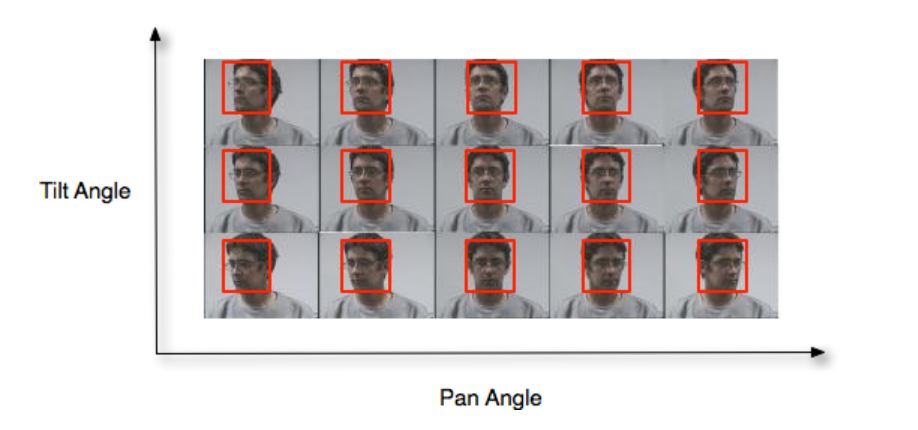
\includegraphics[scale=1]{figures/tiltpan.png}
	\caption{Muestra de 15 fotografías del sujeto 12 \cite{Gourier_Hall_Crowley}}
	\label{fig:img1}
\end{figure}

\begin{figure}[H]
	\centering
	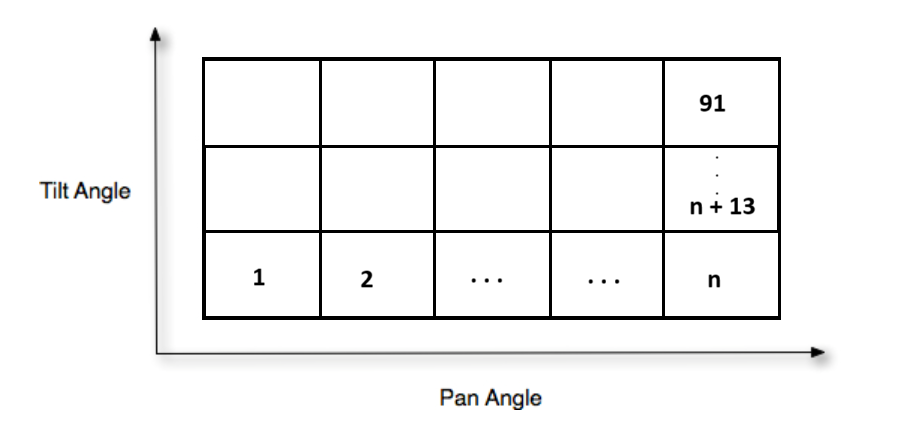
\includegraphics[scale=1]{figures/faceorder.png}
	\caption{Orden de guardado para cada serie de fotografías}
	\label{fig:img2}
\end{figure}

Además de este orden, todas las series de fotografías iniciaban con la imagen de la cabeza completamente hacia arriba y finalizaban con la posición completamente abajo, de frente para ambas. Dado que se tenían 15 sujetos de prueba, se procedió a guardar los archivos JPG de 11 (2046 imágenes) sujetos en un directorio de entrenamiento y los 4 (744 imágenes) restantes en el de pruebas. Al tener en cuenta el orden de los archivos y la cantidad en cada directorio se procedió a realizar las etiquetas por medio de un documento \textit{Excel}con formato \textit{.xlsx}. En dicho documento se creó una hoja para cada grupo de etiquetas, esto quiere decir, una hoja para etiquetas de entrenamiento y otra para etiquetas de prueba. Por lo que, en cada hoja se puede encontrar una columna con las etiquetas en el orden establecido en la Figura 2.

\subsection{Etiquetas para clasificación}

Para la primera experimentación se consideró clasificar las imágenes en 9 clases diferentes, de tal manera que la orientación de la cabeza respecto de la cámara funcionara de manera similar a una palanca de mandos analógica. A continuación se presenta una visualización de dicha clasificación:

\begin{figure}[H]
	\centering
	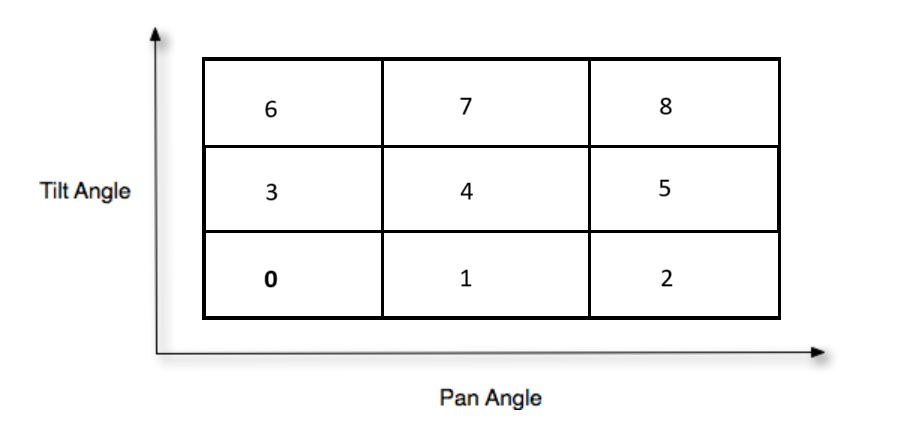
\includegraphics[scale=1]{figures/clasi0.png}
	\caption{Clasificación de imágenes en 9 etiquetas}
	\label{fig:img3}
\end{figure}

Utilizando esta cantidad de clases, se realizaron dos formas de etiquetado en las imágenes, en las cuales solo varía la cantidad de fotografías que fueron etiquetadas dentro de una clase u otra. En las siguientes figuras se podrá observar que la dimensión de cada celda está representada con (n $\times$ m), dónde n corresponde a la cantidad de ángulos panorámicos que abarca y m la cantidad de ángulos de inclinación (según las muestras tomadas del ICPR). Además, la posición de las celdas en las gráficas si corresponde a la numeración de la Figura 2.


\begin{figure}[H]
	\centering
	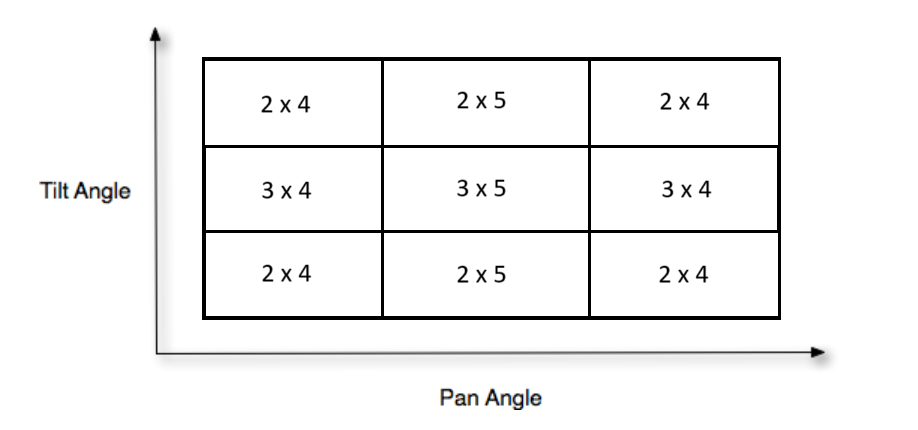
\includegraphics[scale=1]{figures/clasi01.png}
	\caption{Primera distribución de etiquetas}
	\label{fig:img4}
\end{figure}

\begin{figure}[H]
	\centering
	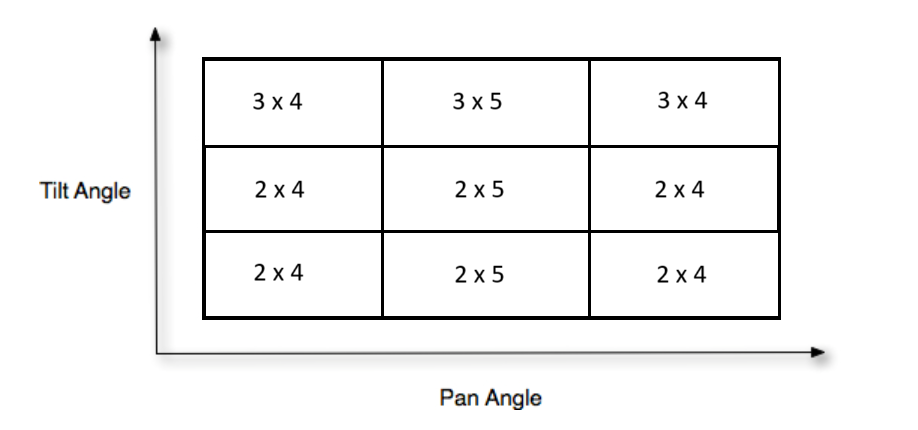
\includegraphics[scale=1]{figures/clasi02.png}
	\caption{Segunda distribución de etiquetas}
	\label{fig:img5}
\end{figure}

Luego de pruebas realizadas con resultados no satisfactorios en la sección de algoritmos para visión por computadora, la siguiente experimentación consistió en reducir la cantidad de clases a 6. En este caso para realizar un movimiento hacia atrás, se requiere un giro completo, en vez del sistema de joystick propuesto anteriormente. La división de clases se muestra a continuación:

\begin{figure}[H]
	\centering
	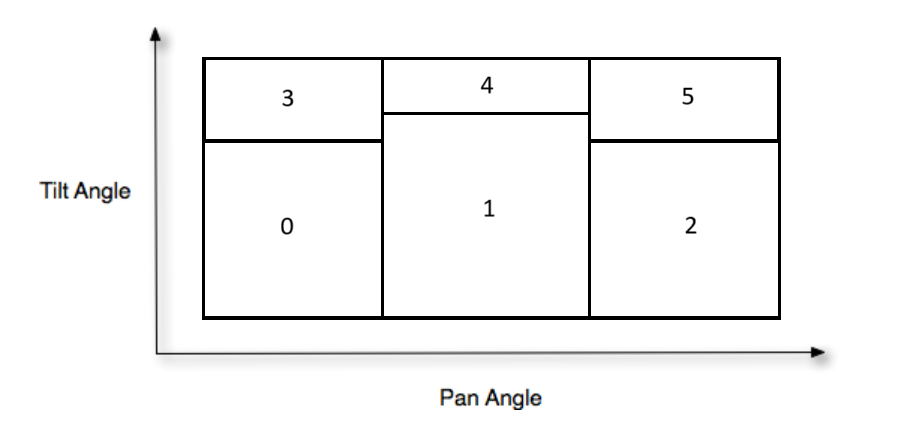
\includegraphics[scale=1]{figures/clasi1.png}
	\caption{Clasificación de imágenes en 6 etiquetas}
	\label{fig:img6}
\end{figure}

\begin{figure}[H]
	\centering
	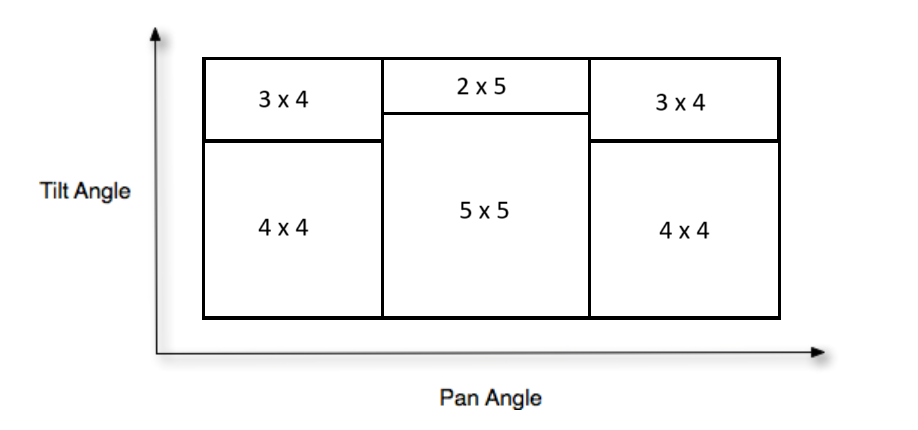
\includegraphics[scale=1]{figures/clasi2.png}
	\caption{Tercera distribución de etiquetas}
	\label{fig:img7}
\end{figure}

\begin{figure}[H]
	\centering
	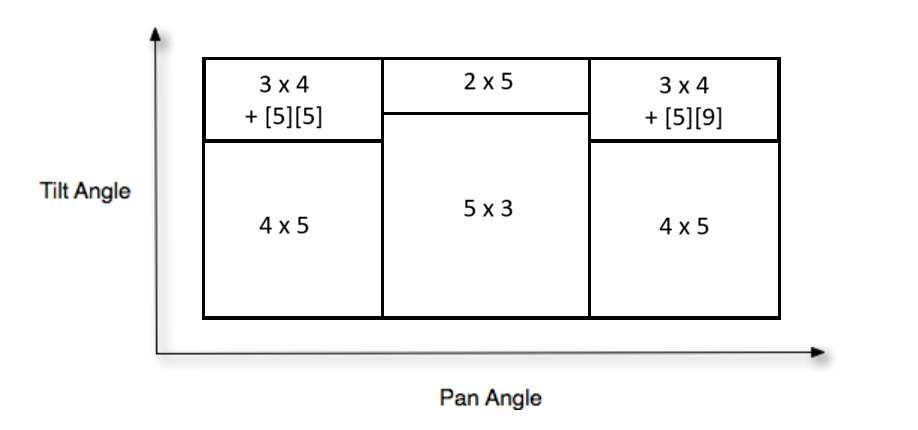
\includegraphics[scale=1]{figures/clasi3.png}
	\caption{Cuarta distribución de etiquetas (Las posiciones se cuentan desde la esquina inferior izquierda)}
	\label{fig:img8}
\end{figure}


\subsection{Fotografías personales}
Dado que los resultados con los modelos de de reconocimiento de orientación no fueron los esperados en ningún caso, se procedió a realizar dos series de fotografías personales con la cámara integrada. Cada serie consta de 9 fotografías con posiciones que simulan las 9 clases inicialmente definidas a una distancia de 45 cm aproximadamente. Una de las series fue tomada en un salón de laboratorio del Departamento de Ingeniería Electrónica, Mecatrónica y Biomédica de la Universidad del Valle de Guatemala y la otra fue realizada en un espacio de trabajo en la casa de Gerardo Andres Fuentes Bámaca (autor). Luego, las fotografías fueron renombradas de tal manera que se pudiera conocer su orden y posición en la lista de imágenes del grupo de entrenamiento. De esta manera, fueron agregadas las etiquetas correspondientes en el documento de etiquetas con extensión \textit{.xlsx}, tanto para los casos de 9 y 6 clases.
\section{ColorFET}
\chapter{Algoritmos para visión por computadora}
\section{Preprocesado de imágenes}


Inicialmente se diseñó un código para extraer fotografías desde un directorio, etiquetas desde un documento con extensión \textit{.xlsx} y luego transformarlos en matrices de datos que para poder ser utilizados en los proceso de \textit{Machine Learning}. Para la realización de este código, se utilizaron las siguientes librerías: \textit{OS}, \textit{CV2 (OpenCV)}, \textit{Numpy} y \textit{Pandas}. Además de esto el proceso para la realización del código fue el siguiente: 

\subsection{Transformación de fotografías}
En este caso, se utilizó la librería \textit{OS} para crear una lista con nombres en formato cadena de los archivos en un directorio dado. Luego, utilizando la librería \textit{Numpy}, se creó una matriz de ceros para guardar todas las fotografías convertidas en formato de matriz. Para realizar la conversión, previamente se realizó una prueba para obtener las dimensiones mínimas con las que puede trabajar la cámara integrada con la librería \textit{CV2}, cuyo tamaño es 320 $\times$ 180 píxeles. Después, dentro de un bucle \textit{for} se utilizó la librería \textit{CV2} obtener la matriz de pixeles de cada fotografía, ajustar el tamaño a las dimensiones encontradas y luego transformar el canal de color por defecto BGR \textit{(Blue, Green, Red)} a RGB \textit{(Red, Green, Blue)}. 

\subsection{Transformación de etiquetas}

Para transformar las etiquetas en matrices de datos, únicamente se requirió la librería \textit{Pandas}, ya que nos permite utilizar una función específica para leer documentos con formato \textit{.xlsx}, así como acceder a las hojas internas del documento. Al guardar el resultado de esta función el siguiente paso es convertirlo a un formato de matriz con funciones de \textit{Numpy}. 

\subsection{Exportación de datos finales}

Antes de realizar la exportación de datos, es importante aplicar una transformación de tipo flotante a entero, en las matrices, y de esta manera se ahorra espacio en el disco duro. Ahora bien, la librería \textit{Numpy} cuenta con una función para exportar matrices de datos de manera individual (una variable a la vez), o bien agruparlas en un solo archivo. En este caso, se guardaron las matrices de fotografías en un solo archivo, dado que estas solo cambiarán si se agregan más fotografías. Por otro lado, las matrices de etiquetas fueron exportadas de manera individual dado que se cuenta con diferentes grupos.

\section{Entrenamiento de modelos de \textit{machine learning}}
Para las primeras pruebas se utilizó el framework \textit{TensorFlow y Keras} para poder realizar los diferentes modelos de \textit{Machine Learning} para reconocimiento de orientación de cabeza, utilizando las matrices de datos obtenidas a partir de la base de datos de ICPR. Para este código se utilizaron las librerías \textit{TensorFlow}, \textit{Matplotlib}, \textit{Numpy} y \textit{Seaborn}. El código fue realizado de la siguiente manera:

\subsection{Extracción de datos previamente procesados}
Luego de exportar los archivos transformados de la base de datos, se generan archivos con extensión \textit{.npy} para los archivos de una variable y \textit{.npz} para los de múltliple variables. Dichos archivos pueden ser importados utilizando también funciones de la librería \textit{Numpy}, para guardarlos en variables utilizables dentro del código, optimizando así el tiempo de transformación de datos.

\subsection{Modelo de reconocimiento de orientación de cabeza}
El primer pasó fue normalizar los valores de las matrices, dado que son imágenes RGB, cada píxel de estas está representado por 3 valores que varían entre 0 y 255, y se necesitan valores entre 0 y 1, por lo que únicamente se tuvo que dividir tanto la variable con datos de entrenamiento y prueba entre el valor 255. 

Inicialmente, dado que se trata de un modelo que trabaja con matrices derivadas de fotografías, se utilizó una CNN (Red Convolucional Neurnal), la cual permite detectar patrones en las imágenes. Utilizando \textit{Tensorflow} y \textit{Keras}, se definieron 7 capas para la generación del modelo. En este caso se utilizó en primera instancia una capa convolucional en 2D, con 10 kernels de tamaño 3 $\times$ 3, función de activación \textit{ReLU}, y por ser la primera capa se agregan las dimensiones de entrada (fotografía). Luego, se aplicó una capa con la técnica de \textit{Max Pooling} con tamaño 2 $\times$ 2. Después, se aplica una capa de aplanado previa necesaria para poder utilizar las siguientes capas densas. Esta vez se utilizaron 3 capas densas, con 75, 150 y 75 nodos respectivamente con función de activación \textit{ReLU}. Por último, se aplica una capa densa con una cantidad de nodos definida por el número de clases a utilizar y función de activación \textit{Softmax}. Con esta especificación de hiperparámetros, se procede a unir las capas en un modelo secuencial, para luego compilarlo con un optimizador \textit{Adam}, para la pérdida se utilizó \textit{Sparse categorical crossentropy}, dado que las etiquetas fueron definidas como enteros y no en el formato \textit{One-Hot}. Para finalizar con los hiperparámetros, en la opción métricas se escoge la opción \textit{Accuracy} o precisión. Luego de entrenado el modelo, se procede a guardarlo con la función de guardar en \textit{Keras}, en el cual el argumento es el directorio donde se desea guardar el archivo con extensión \textit{.keras} y poder utilizarlo en otros códigos.

Al tener configurado el modelo, se procede al entrenarlo, guardarlo y exportar las gráficas descriptivas respectivas. En esta etapa se cuenta con 4 modelos que varían dado que se utilizó cada uno de los diferentes grupos de etiquetas. A continuación se muestran las gráficas de pérdida y exactitud para cada modelo, utilizando el grupo de entrenamiento actualizado con las fotografías de Gerardo Fuentes (autor), así como las matrices de confusión utilizando la librería \textit{Seaborn}:

\begin{figure}[H]
	\centering
	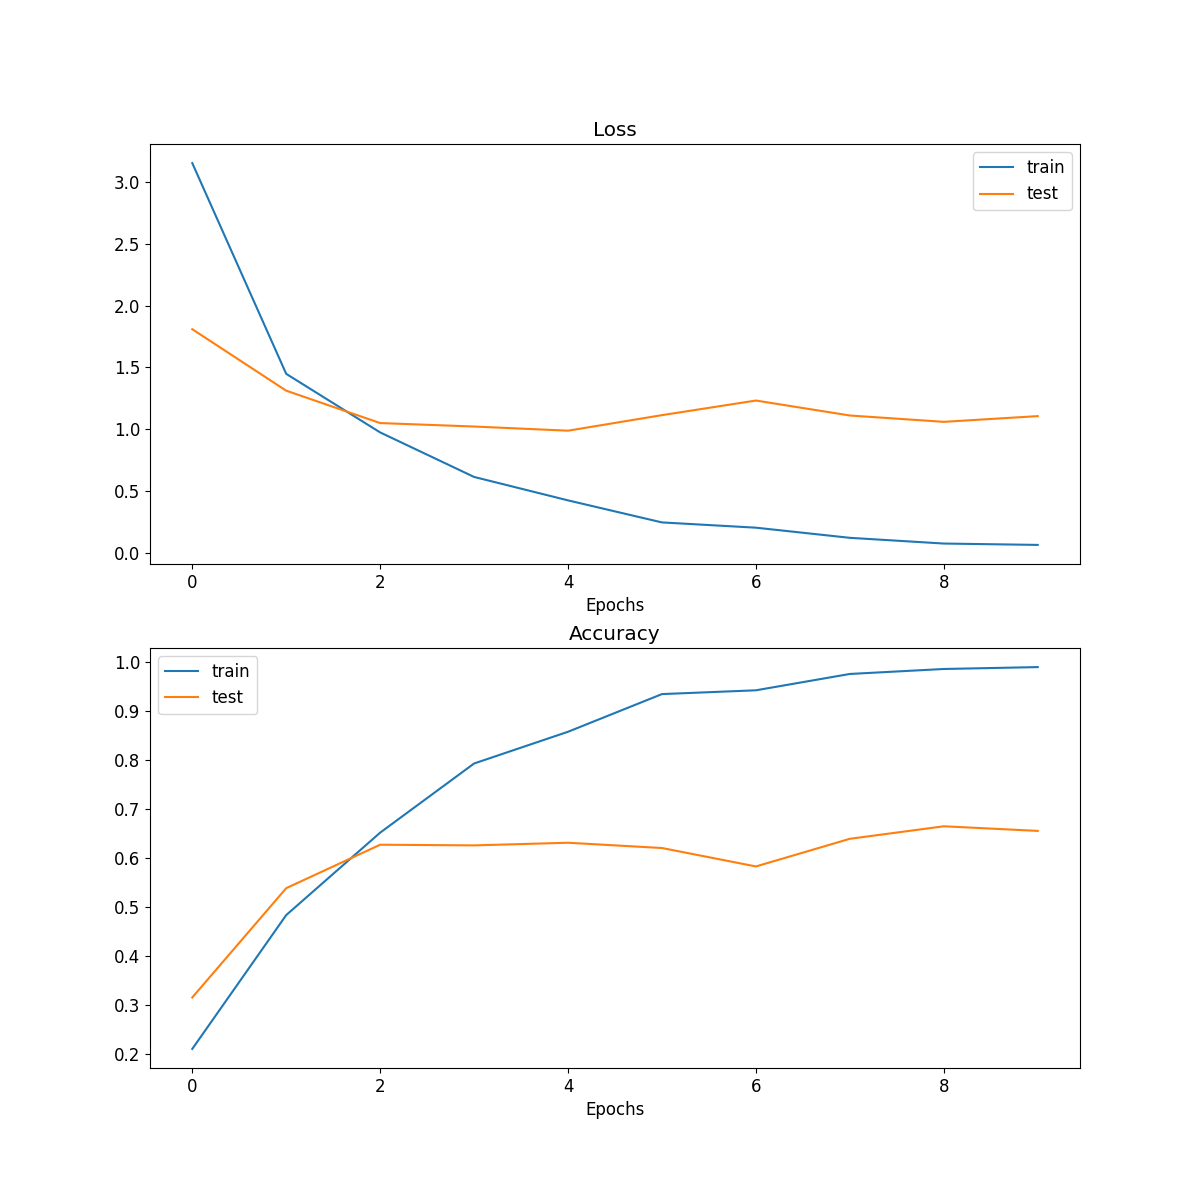
\includegraphics[scale=0.65]{figures/LA0.png}
	\caption{Pérdida y exactitud del primer modelo con 9 clases}
	\label{fig:img9}
\end{figure}

\begin{figure}[H]
	\centering
	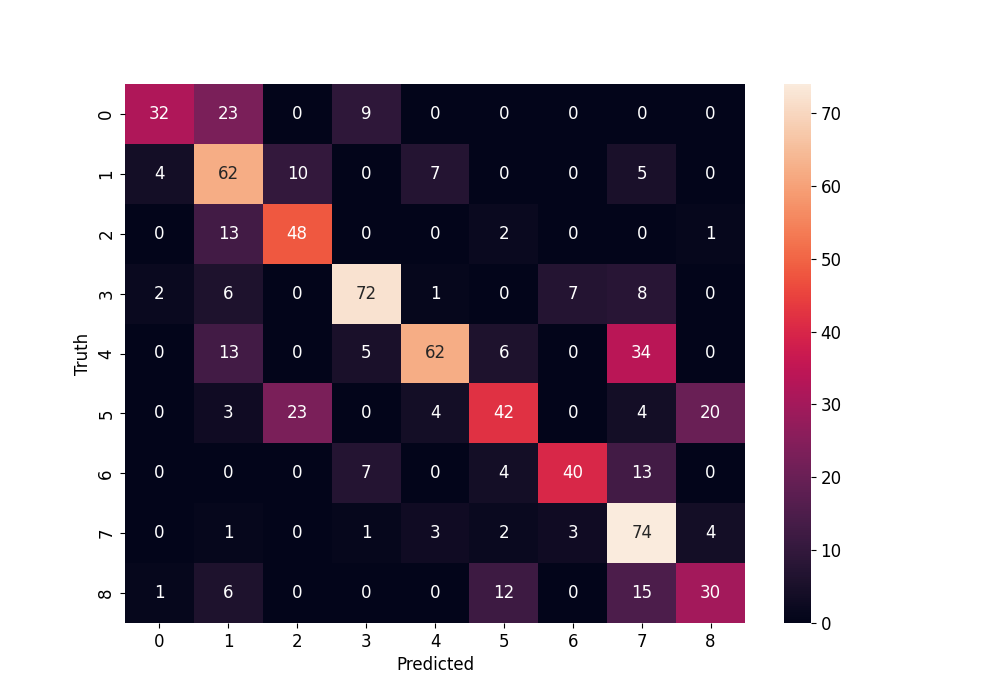
\includegraphics[scale=0.75]{figures/CM0.png}
	\caption{Matriz de confusión del primer modelo con 9 clases}
	\label{fig:img10}
\end{figure}

\begin{figure}[H]
	\centering
	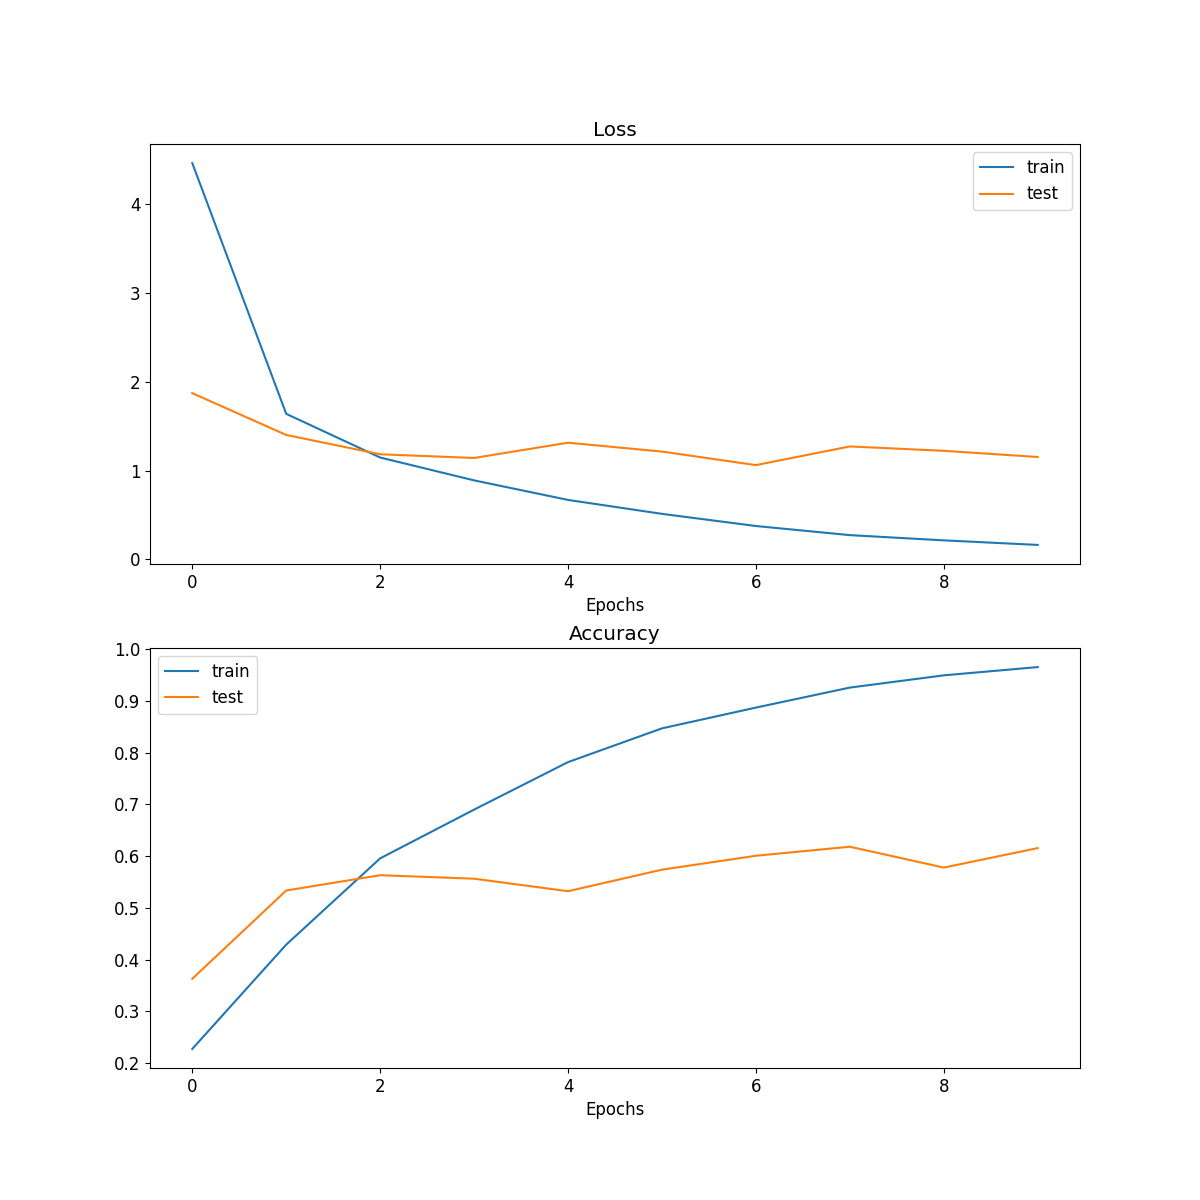
\includegraphics[scale=0.65]{figures/LA1.png}
	\caption{Pérdida y exactitud del segundo modelo con 9 clases}
	\label{fig:img11}
\end{figure}

\begin{figure}[H]
	\centering
	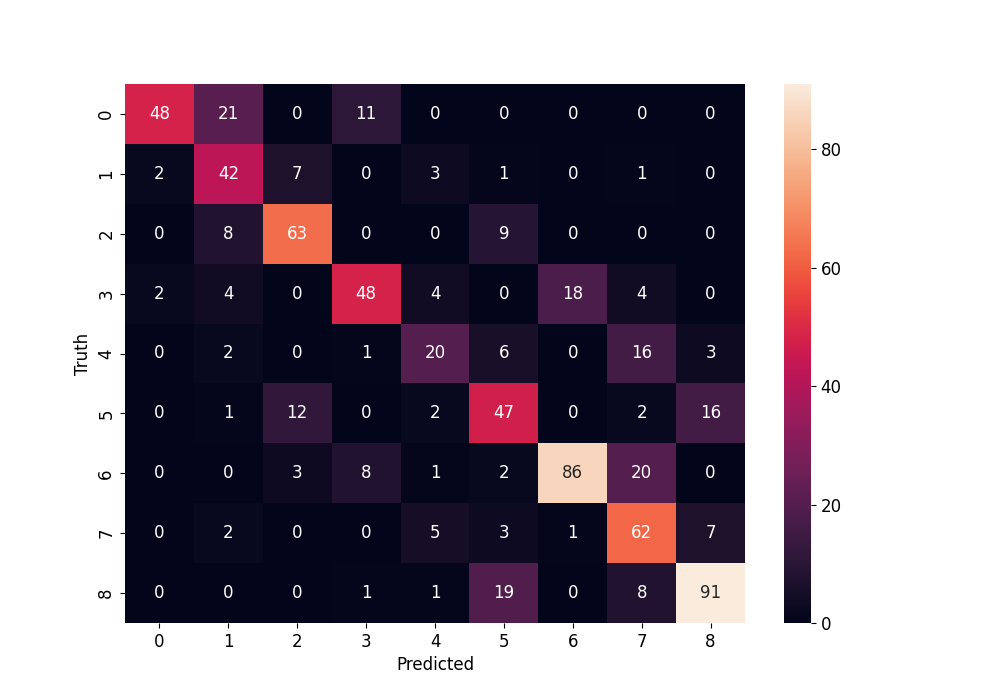
\includegraphics[scale=0.75]{figures/CM1.png}
	\caption{Matriz de confusión del segundo modelo con 9 clases}
	\label{fig:img12}
\end{figure}

\begin{figure}[H]
	\centering
	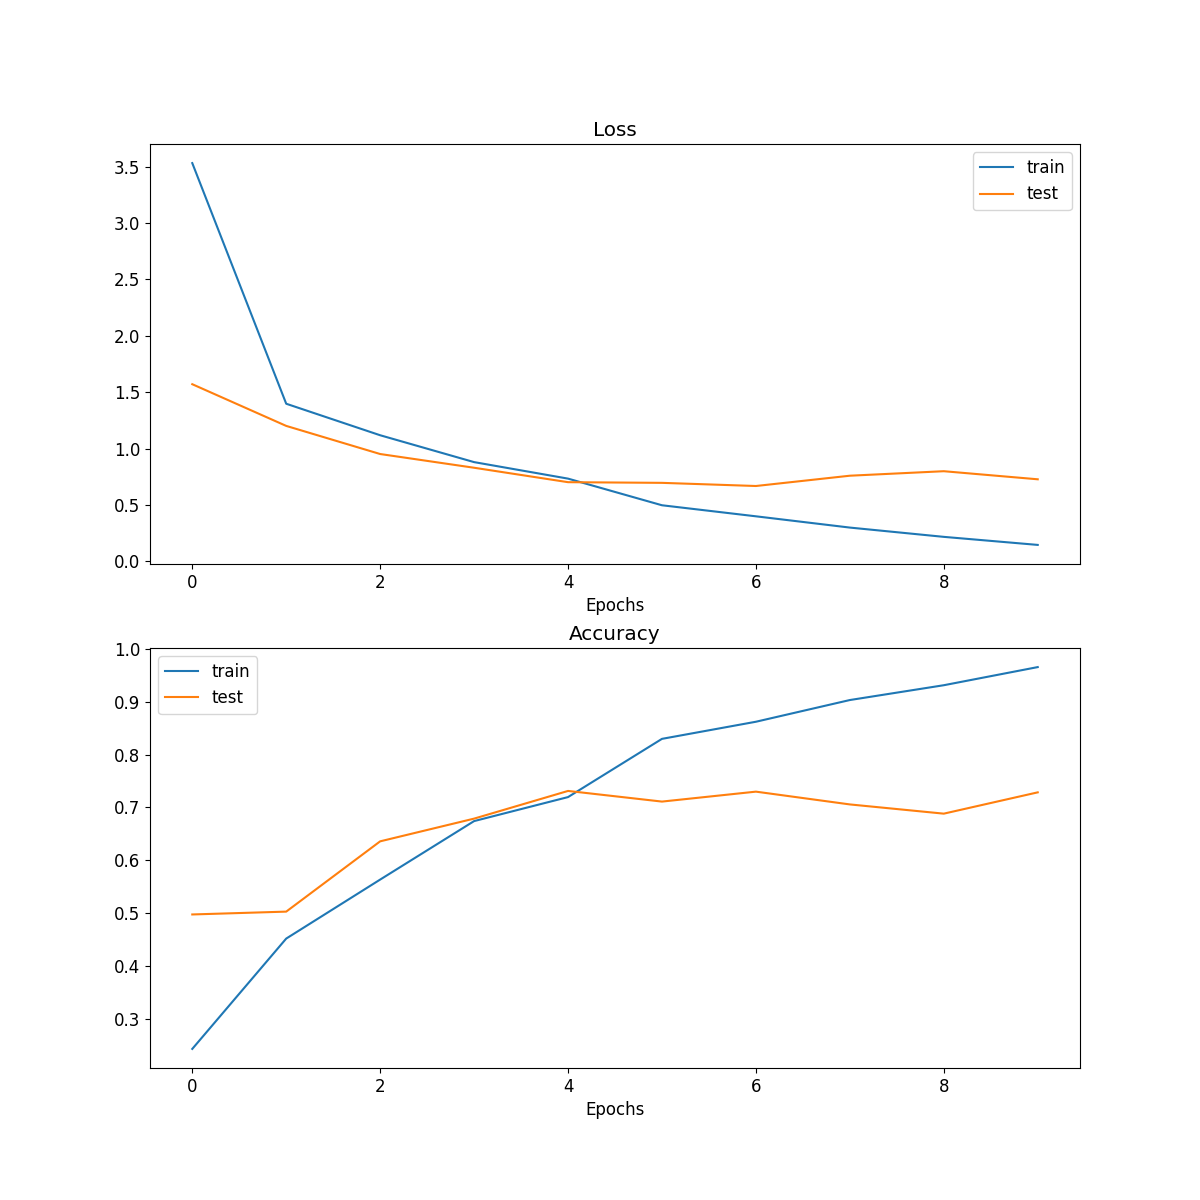
\includegraphics[scale=0.65]{figures/LA2.png}
	\caption{Pérdida y exactitud del primer modelo con 6 clases}
	\label{fig:img13}
\end{figure}

\begin{figure}[H]
	\centering
	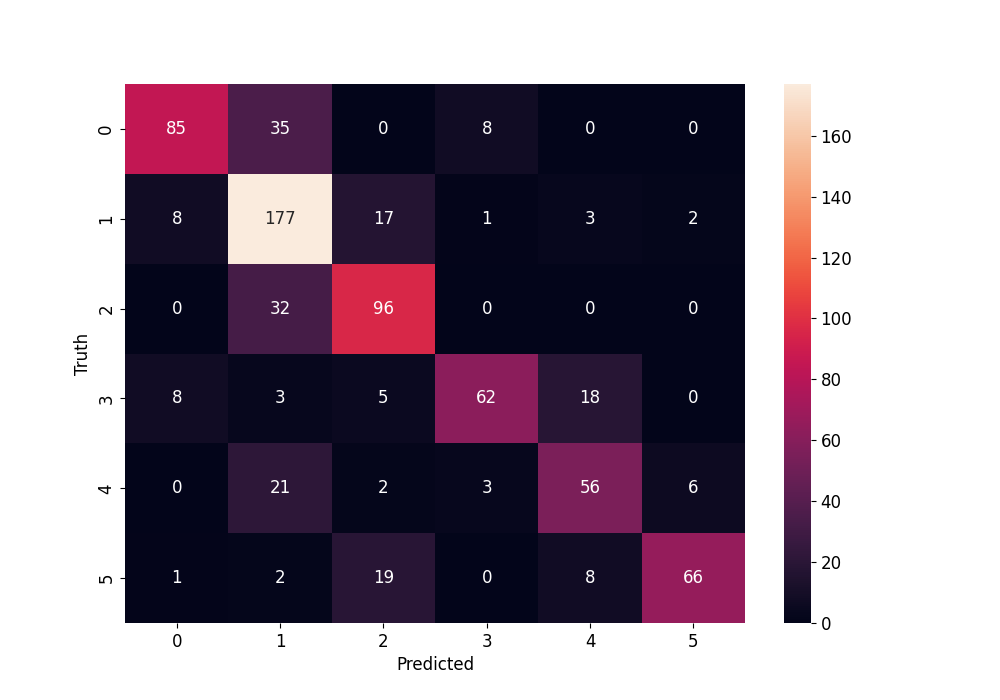
\includegraphics[scale=0.75]{figures/CM2.png}
	\caption{Matriz de confusión del primer modelo con 6 clases}
	\label{fig:img14}
\end{figure}

\begin{figure}[H]
	\centering
	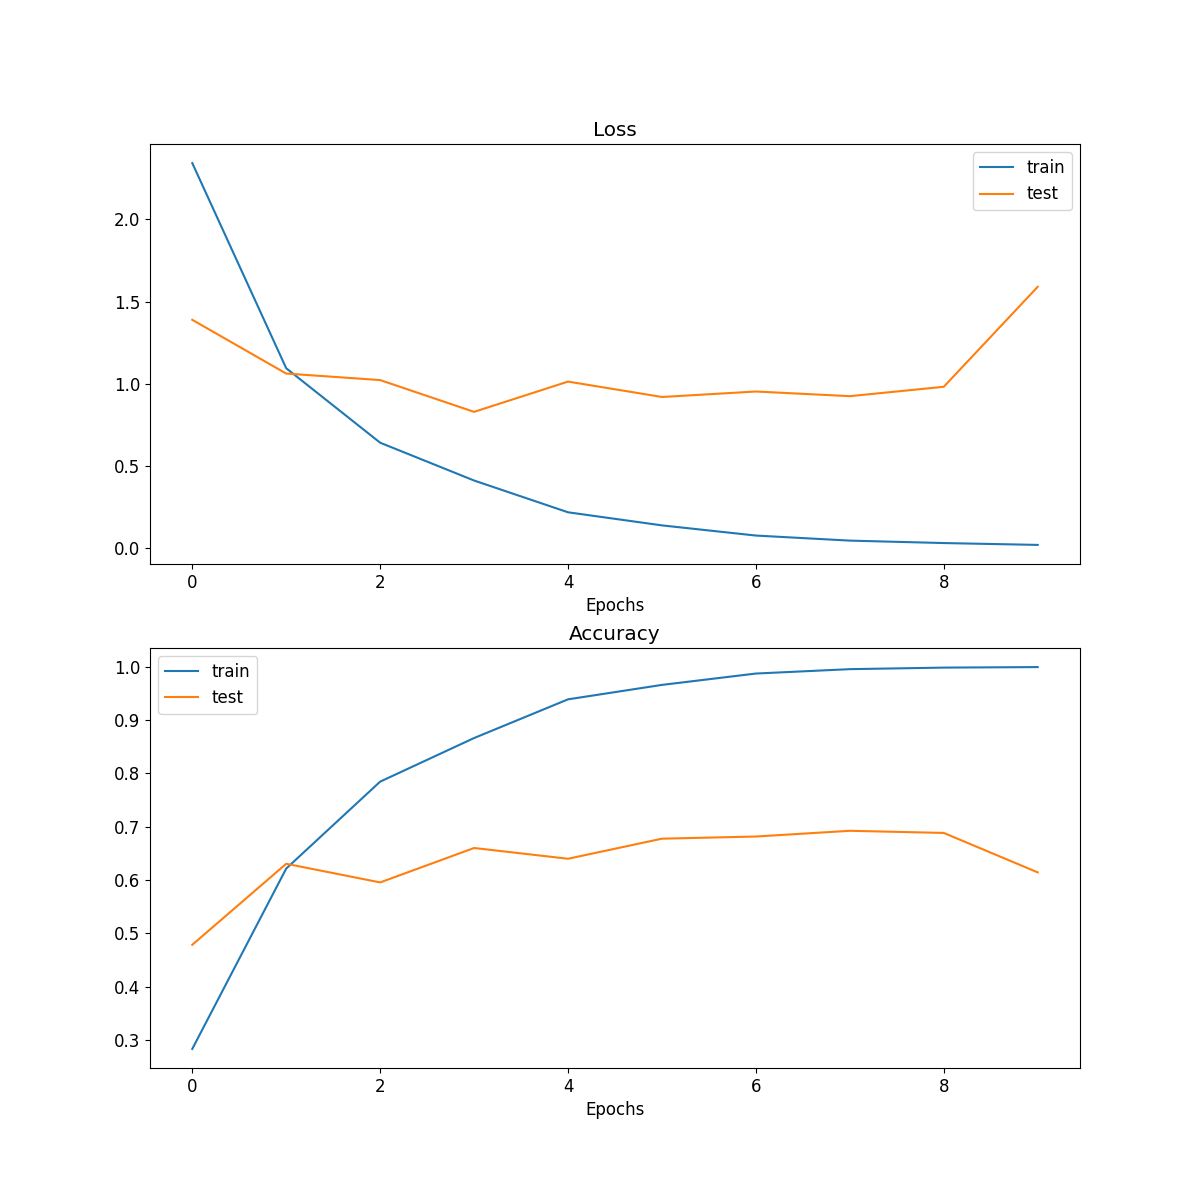
\includegraphics[scale=0.65]{figures/LA3.png}
	\caption{Pérdida y exactitud del segundo modelo con 6 clases}
	\label{fig:img15}
\end{figure}

\begin{figure}[H]
	\centering
	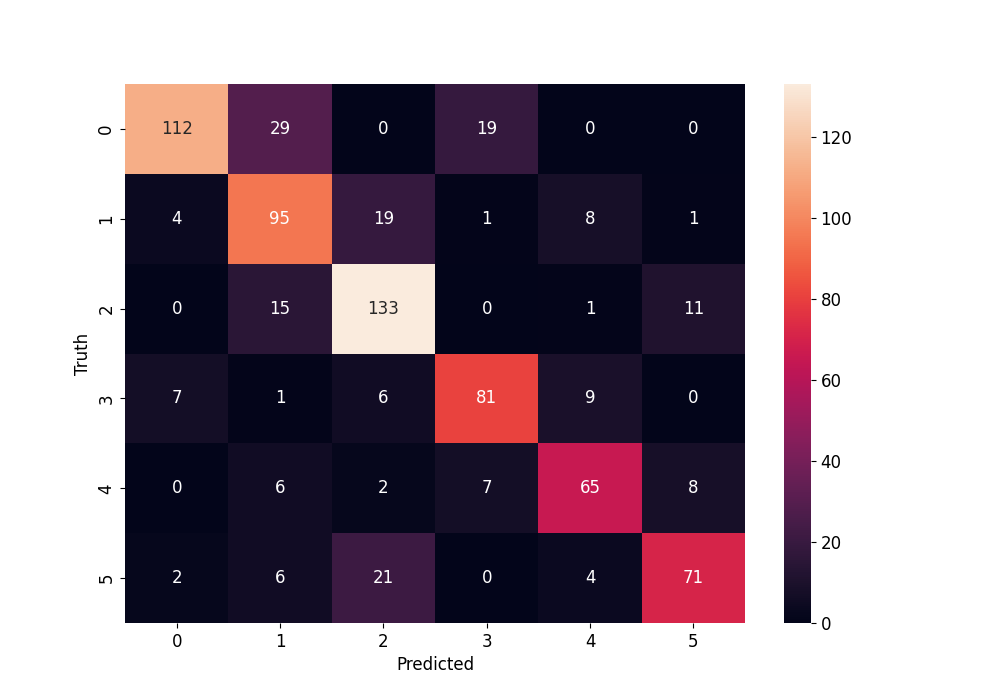
\includegraphics[scale=0.75]{figures/CM3.png}
	\caption{Matriz de confusión del segundo modelo con 6 clases}
	\label{fig:img16}
\end{figure}

En las figuras 9 a las 16 se puede observar que se produce un sobreajuste en todos los modelos entrenados, el cual sucede dado que las fotografías de la base de datos ICPR, tienen el mismo fondo en todos su casos. Además, la mayoría de los sujetos de prueba son de sexo masculino, caucásicos y con un rango de edad similar. Además de ser únicamente 11 personas diferentes. Con dichos resultados, se pueden tomar diferentes decisiones. Las acciones a considerar son: 

\begin{itemize}
	\item Conseguir más fotografías y con más diversidad de sujetos y fondos.
	\item Reducir nuevamente la cantidad de clases a 3 o 4. 
	\item Realizar un sobreajuste enfocado en el rostro del usuario.
\end{itemize}


\section{Ajuste de modelos preentreanados}
\section{Pruebas en tiempo real}

Para las primeras pruebas se utilizaron los 4 modelos exportados, la cámara integrada y un bucle infinito. En este caso es utilizaron las siguientes librerías \textit{CV2}, \textit{TensorFlow} y \textit{Numpy}. El primer paso de la configuración fue cargar el modelo previamente exportado. Luego, se realiza la inicialización de la cámara integrada por medio de \textit{OpenCV}, y se ajusta el tamaño de la imagen a obtener por medio de comandos de la librería \textit{CV2}. 
Ahora bien, en el bucle infinito se realiza una captura de la imagen obtenida por la cámara, la cual se guarda como una matrices de píxeles. Luego, se cambia el canal de BGR a RGB, se normaliza la matriz al dividirla entre 255, y se cambia la matriz de tipo flotante a entero. Después, por medio de la librería \textit{TensorFlow} se utiliza la función Predecir, la cual devuelve una vector con el porcentaje de similitud predecido para cada clase. Finalmente, se aplica la función de \textit{Numpy} para obtener el valor más máximo dentro de dicho vector de predicciones y dicho valor se imprime en la consola.
Al realizar dicho proceso, se comprobó que los resultados de las gráficas descriptivas de los modelos entrenados son congruentes, dado que los resultados no fueron satisfactorios al detectar las posiciones inferior izquierda de la cabeza y la alta fluctuación entre las posiciones centrales.

%Esta etapa contempla la iteración de pruebas para conseguir un algoritmo que funcione de manera efectiva al reconocer los gestos y movimientos de la cabeza del usuario. Luego de obtener un reconocimiento efectivo, se generarán diferentes ítems, clases o divisiones para cada tipo de gestos. Al tener definida la lista de tipos, se procede a utilizarlos para generar comandos genéricos para poder utilizar los agentes robóticos móviles simulados y físicos.

\chapter{Simulaciones}

%El algoritmo anterior será utilizado para realizar simulaciones de movimiento/envío de comandos en diferentes escenarios. Para poder ejecutar dichas pruebas, será necesario también realizar un análisis de los diferentes simuladores disponibles, los cuales sean compatibles con los algoritmos determinados anteriormente. Se realizará un registro de datos de las iteraciones realizadas para analizarlas de manera estadísticas y determinar el comportamiento de cada algoritmo según el escenario propuesto. De esta manera, se podrá partir con datos o comandos iniciales para las pruebas físicas. Los escenarios a probar constan del entorno físico alrededor del robot, así como los diferentes gestos a utilizar. 

\chapter{Pruebas físicas}

%Al obtener los parámetros iniciales determinados en las simulaciones, se empezará la migración de estos, junto con los algoritmos, hacia los robots a utilizar. En primer lugar se realizará una comparación entre los resultados obtenidos de manera física contra las simulaciones. Las pruebas físicas se realizarán en diferentes condiciones, como el de luminosidad, o el de contenido visual con diferentes niveles de ruido para tener un rango de operación más grande. También, las pruebas físicas tendrán un análisis cada algoritmo con diferentes variaciones en parámetros iniciales o en el algoritmo por sí mismo. De esta manera se podría verificar el alcance del sistema en conjunto, del robot, el sensor y el algoritmo seleccionado. También, se realizarán pruebas con diferentes sujetos de control, es decir diferentes personas realizando los gestos para controlar el movimiento del robot. Al realizar las pruebas, también se guardaran los datos obtenidos a partir de los sensores de tal manera que se puedan clasificar dependiendo del gesto utilizado. 
